\documentclass[11pt]{article}
\usepackage[margin=1.9cm]{geometry}
\usepackage{booktabs}
\usepackage{graphicx}
\usepackage{xcolor}
\usepackage{enumitem}
\usepackage[hidelinks]{hyperref}
\usepackage{titlesec}
\usepackage{fancyhdr}
\usepackage{tabularx}
\usepackage{framed}


% ---------- palette ----------
\definecolor{native}{HTML}{0F9D58}
\definecolor{mcp}{HTML}{4285F4}
\definecolor{plainc}{HTML}{9AA0A6}
\definecolor{ink}{HTML}{1A1A1A}
\definecolor{rule}{HTML}{D8D8D8}
\definecolor{panelbg}{HTML}{F4F8F4}     % faint green panel
\definecolor{panelln}{HTML}{0F9D58}
\definecolor{greybg}{HTML}{F2F2F2}
\definecolor{amber}{HTML}{C9A227}

% ---------- type ----------
\titleformat{\section}{\large\bfseries\color{ink}}{\thesection}{0.55em}{}
\titlespacing{\section}{0pt}{12pt}{4pt}
\titleformat{\subsection}{\normalsize\bfseries\color{ink}}{}{0em}{}
\titlespacing{\subsection}{0pt}{8pt}{2pt}
\setlist{nosep,leftmargin=1.3em}
\renewcommand{\arraystretch}{1.15}

\pagestyle{fancy}\fancyhf{}
\lhead{\small\color{plainc}Graph-Native Coding Harness}
\rhead{\small\color{plainc}\thepage}
\renewcommand{\headrulewidth}{0.3pt}

\newcommand{\native}[1]{\textcolor{native}{\textbf{#1}}}
\newcommand{\mcp}[1]{\textcolor{mcp}{\textbf{#1}}}

% caption styling without the caption package
\makeatletter
\renewcommand{\fnum@figure}{\textbf{\figurename~\thefigure}}
\renewcommand{\fnum@table}{\textbf{\tablename~\thetable}}
\long\def\@makecaption#1#2{\vskip 3pt\centering\footnotesize\textcolor{plainc}{#1.\ #2}\par}
\makeatother

% ---------- KEY-FINDING banner (green left rule + tint) ----------
\newenvironment{keyfind}{%
  \def\FrameCommand{\color{panelln}\vrule width 3pt\hspace{8pt}%
    \fboxsep=8pt\colorbox{panelbg}}%
  \MakeFramed{\hsize\dimexpr\linewidth-11pt\relax\FrameRestore}}{\endMakeFramed}

% ---------- light callout (grey) for caveats ----------
\newenvironment{caveat}{%
  \def\FrameCommand{\color{rule}\vrule width 2pt\hspace{8pt}\fboxsep=7pt\colorbox{greybg}}%
  \MakeFramed{\hsize\dimexpr\linewidth-9pt\relax\FrameRestore}\small}{\endMakeFramed}

% ---------- HERO number tile ----------
\newcommand{\herotile}[3]{% color, big number, label
  \begin{minipage}[t]{0.31\linewidth}\centering
  \colorbox{#1!12}{\parbox[t][2.0cm][c]{\linewidth}{\centering
    {\fontsize{30}{32}\selectfont\textcolor{#1}{\textbf{#2}}}\\[2pt]
    {\footnotesize\color{ink} #3}}}\end{minipage}}

% ---------- manual figure numbering (so hand-placed images + captions don't collide) ----------
\newcounter{fig}
\newcommand{\figcap}[1]{\refstepcounter{fig}\par\vspace{2pt}{\footnotesize\color{plainc}\textbf{Figure \thefig.} #1}\par}

% ---------- trace step ----------
\newcommand{\stp}[3]{\item[\textcolor{plainc}{\footnotesize\sffamily #1}]{\small\texttt{#2}}\ \ {\footnotesize #3}}
\newenvironment{trace}{\begin{list}{}{\setlength{\leftmargin}{2.0em}\setlength{\labelwidth}{1.6em}%
  \setlength{\itemsep}{1.5pt}\setlength{\topsep}{3pt}}}{\end{list}}

\begin{document}
\thispagestyle{empty}

% ===================== TITLE =====================
\begin{center}
{\fontsize{22}{24}\selectfont\bfseries\color{ink} Graph-Native Coding Harness}\\[3pt]
{\large\color{ink} Does giving a coding agent a code graph actually help --- and \emph{how} should it be wired in?}\\[6pt]
{\footnotesize\color{plainc} Benchmarked on \texttt{Graph-Query-Engine} (24k LOC React/Vite + Python Flask) \,$\bullet$\,
3 harnesses on \texttt{claude -p} \,$\bullet$\, quality scored by a blind LLM judge}
\end{center}
\vspace{2pt}{\color{rule}\hrule height1pt}\vspace{10pt}

% ===================== HERO FINDING =====================
\begin{keyfind}
{\large\textbf{The finding.}}\ \ Across six hard, diverse tasks, \native{graph-native}---which has the
harness \emph{rank the relevant code and inject it before the agent's first token}---delivers the
\native{best average quality} \emph{and} the \native{lowest cost}. But \textbf{no single harness wins
everything}: the right way to wire in the graph \emph{depends on the task}.
\end{keyfind}

\vspace{8pt}
\begin{center}
\herotile{native}{8.97}{mean quality / 10\\(best of 3 harnesses)}\hfill
\herotile{native}{8.2}{quality per dollar\\(most cost-efficient)}\hfill
\herotile{ink}{4 / 6}{tasks won or tied\\by graph-native}
\end{center}

\vspace{10pt}
% ===================== THREE-WAY ONE-LINER =====================
\noindent\textbf{Who wins what} (the one thing to remember):
\begin{center}\small
\begin{tabularx}{\linewidth}{@{}p{3.1cm} >{\raggedright\arraybackslash}X@{}}
\native{graph-native} wins & \textbf{structured-traversal} tasks --- data-flow tracing, API migration (the answer is a known walk over the graph). \\
\mcp{graph-MCP} wins & \textbf{open-ended} tasks --- bug diagnosis, security audit (interactive querying beats a fixed up-front list). \\
\textcolor{plainc}{\textbf{plain}} competes & only on \textbf{thorough-sweep} tasks where brute-force reading already suffices. \\
\end{tabularx}
\end{center}

\vspace{6pt}
\begin{center}
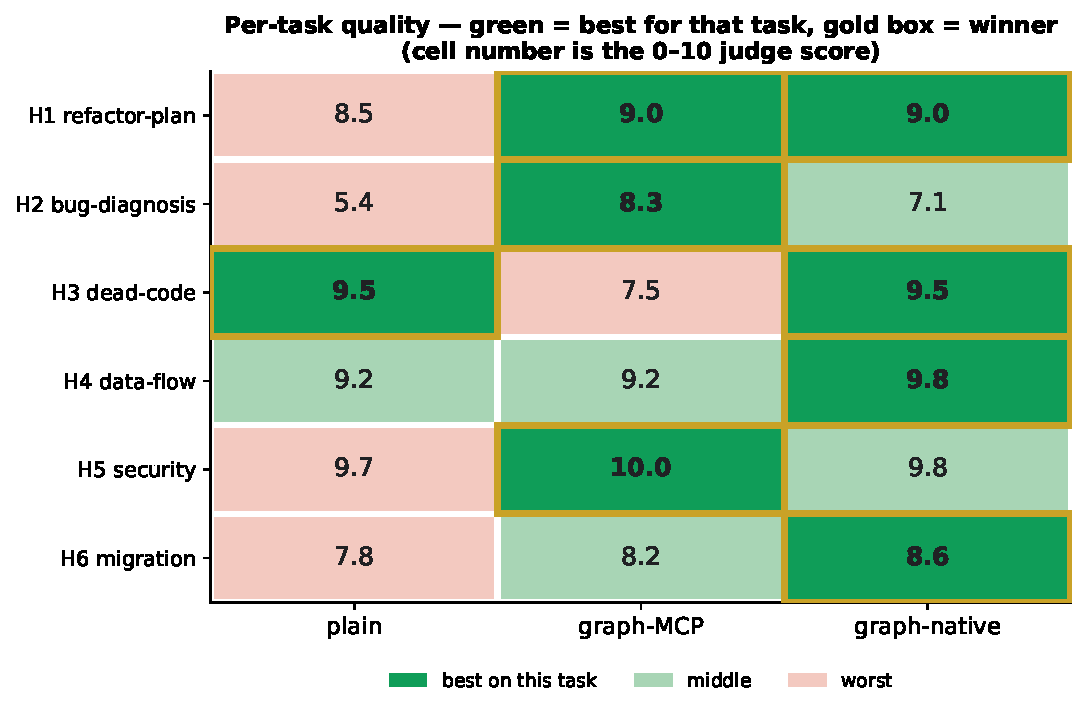
\includegraphics[width=0.97\linewidth]{figs/heatmap.pdf}
\end{center}
\figcap{Per-task quality. Green = best harness for that task, gold box = winner; the cell number is
the 0--10 judge score. The point is the \emph{mixed} pattern --- a benchmark where one column was
always green would be rigged.}

\clearpage
% ===================== THE THREE HARNESSES =====================
\section{What the three harnesses are}
The only thing that differs is \textbf{where retrieval and ranking happen} --- same model
(\texttt{claude -p}), same tasks, same budget.

\begin{center}\small
\begin{tabularx}{\linewidth}{@{}p{2.6cm} p{3.2cm} >{\raggedright\arraybackslash}X@{}}
\toprule
\textbf{Harness} & \textbf{Tools} & \textbf{Where retrieval happens} \\
\midrule
\textcolor{plainc}{\textbf{plain}} & Read / Grep / Bash & \emph{In the agent} --- it greps and reads to discover the relevant code. \\
\mcp{graph-MCP} & + codegraph MCP & \emph{In the agent, on demand} --- it queries the graph mid-reasoning, hop by hop. \\
\native{graph-native} & + ranked injection & \emph{In the harness, before turn 0} --- a ranked, test-demoted file list is injected up front; the agent only verifies it. \\
\bottomrule
\end{tabularx}
\end{center}

\begin{keyfind}
\textbf{The mechanism, in one line.} The graph's value is realized by \emph{relocating ranking out of
the model's context and into deterministic harness code} --- not by exposing a better tool.
\end{keyfind}

% ===================== QUALITY RESULTS =====================
\section{Quality --- judged blind by an independent \texttt{claude -p}}
Six tasks, each a different \emph{kind} of work (refactor plan, bug diagnosis, dead-code safety,
data-flow trace, security audit, API migration). Each answer is graded 0--10 on a per-task rubric by
a fresh \texttt{claude -p} with \textbf{no tools and no repo access}, with answers fenced as data and
labeled A/B/C so it cannot tell which harness produced them.

\begin{center}
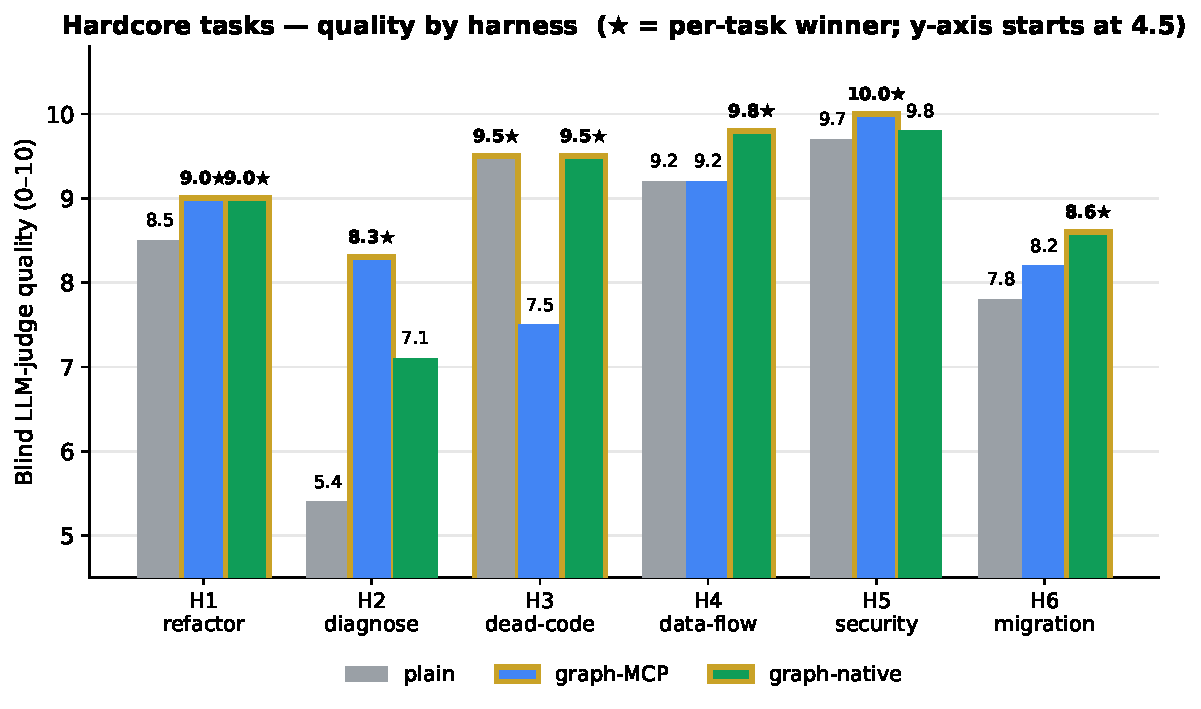
\includegraphics[width=0.97\linewidth]{figs/hardcore_quality.pdf}
\end{center}
\figcap{Quality by harness across the six tasks (gold ring + $\star$ = per-task winner; the y-axis
starts at 4.5 so the spread is visible). plain collapses on the cross-file bug trace (H2: 5.4).}

\vspace{6pt}
\begin{center}
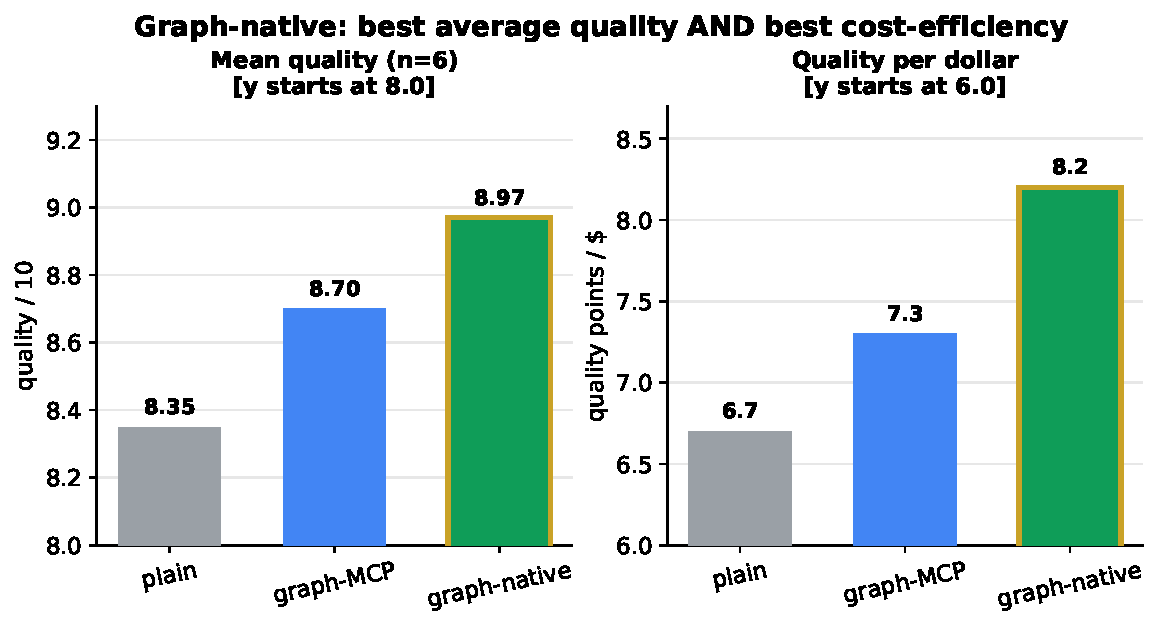
\includegraphics[width=0.9\linewidth]{figs/quality_per_dollar.pdf}
\end{center}
\figcap{The dual win: graph-native is both the highest-quality \emph{and} the most cost-efficient
harness (both panels use a zoomed y-axis, noted in their titles, so the gaps are legible).}

\vspace{8pt}
% ===================== THE TRACE — actual process =====================
\section{How each harness actually worked (case study: the H2 bug diagnosis)}
We re-ran the bug-diagnosis task (``why does expanding the graph reset the zoom?'') with full
streaming traces and recorded the \textbf{literal sequence of tool calls} each harness made. This is
the mechanism made concrete --- not a description, the captured play-by-play.

\begin{center}\small
\begin{tabular}{lcccccc}
\toprule
 & \textbf{turns} & \textbf{tools} & Read & Grep & Bash & Skill \\
\midrule
\textcolor{plainc}{\textbf{plain}} & 18 & 16 & 7 & \textbf{6} & 2 & 1 \\
\mcp{graph-MCP} & 18 & 16 & 8 & \textbf{6} & 1 & 1 \\
\native{graph-native} & \native{\textbf{14}} & \native{\textbf{12}} & 8 & \native{\textbf{2}} & 1 & 1 \\
\bottomrule
\end{tabular}
\end{center}

\subsection{\textcolor{plainc}{plain} --- discovers the code by searching}
\begin{trace}
\stp{1--2.}{Skill, Read}{invoke systematic-debugging; \emph{open \texttt{CODE\_GRAPH.md}} to localize.}
\stp{3--4.}{Read $\times$2}{read the renderer + panel; find the \texttt{ResizeObserver $\to$ resetView} path.}
\stp{5--9.}{Grep $\times$3, Read}{hunt \texttt{resetView|pageCluster|.fit(} to trace the ``+ more'' routing.}
\stp{10--16.}{Bash, Read, Grep $\times$4}{\texttt{git log} finds a prior fix; final greps confirm no viewport-capture helper exists.}
\stp{$\Rightarrow$}{}{quality \textbf{5.4} --- right family of answer, most churn, least precise.}
\end{trace}

\subsection{\mcp{graph-MCP} --- pulls the code on demand}
\begin{trace}
\stp{1--2.}{Skill, Read}{invoke skill; read \texttt{CODE\_GRAPH.md} (repo mandates it).}
\stp{3--6.}{Grep $\times$2, Read $\times$2}{find every \texttt{cy.(zoom|pan|fit)} call; flag the \texttt{ResizeObserver} + \texttt{isMore} handler.}
\stp{7--13.}{Grep $\times$3, Read $\times$3, Bash}{trace the exact ``+ more'' tap path; \texttt{git log} finds the prior \#9 fix.}
\stp{14--16.}{Read $\times$2, Grep}{confirm no zoom/pan-preservation exists --- the conclusive evidence.}
\stp{$\Rightarrow$}{}{quality \mcp{8.3} (best) --- enumerated \emph{every} \texttt{fit()} path + a full 10-item re-test list.}
\end{trace}

\subsection{\native{graph-native} --- is handed the code, then verifies}
\begin{trace}
\stp{1.}{Skill}{invoke systematic-debugging.}
\stp{2.}{Read}{\textbf{skips \texttt{CODE\_GRAPH.md}} --- the injected list already named the surface, so it goes \emph{straight} to the panel.}
\stp{3.}{Grep}{\emph{one} targeted grep to find the pagination entry.}
\stp{4--9.}{Read $\times$6}{walk the renderer: confirm \texttt{pageCluster} is fixed, find \texttt{toggleCluster}/\texttt{toggleNodeExpansion} call \texttt{cy.fit()} (the live bug).}
\stp{10--12.}{Grep, Read, Bash}{\emph{second and last} grep to confirm the architecture; read tests; \texttt{git log}.}
\stp{$\Rightarrow$}{}{quality \textbf{7.1} --- \native{fewest turns (14) and only 2 greps}: it verified the map instead of discovering it.}
\end{trace}

\begin{keyfind}
\textbf{What the traces show.} plain and graph-MCP both \emph{open by reading \texttt{CODE\_GRAPH.md},
then run a 6-grep hunt} to discover the change surface. graph-native \emph{skips discovery entirely}
and uses \native{2 greps to verify} --- 4 fewer searches, 4 fewer turns, because the harness already
did the retrieval. \emph{That is the efficiency win, observed literally.}
\end{keyfind}

\begin{caveat}
\textbf{Honest caveat.} In this captured run the \mcp{graph-MCP} agent did \emph{not} fire its
\texttt{codegraph\_*} tools --- it solved H2 with text search like plain, so its measured tool profile
matches plain's (tool use is non-deterministic; its 8.3 win came from thoroughness here). The contrast
that reproduces deterministically is graph-native's skipped discovery loop.
\end{caveat}

\clearpage
% ===================== SUPPORTING EVIDENCE =====================
\section{Supporting evidence}

\subsection{A deterministic retrieval oracle (n=8), validated live}
Before scoring agents, we measured what each harness \emph{can deliver} --- a fast, reproducible
file-localization F1 over 8 retrieval tasks. The ordering matches the quality results, and a live
\texttt{claude -p} A/B confirmed it on the hardest case.

\begin{minipage}{0.52\linewidth}\centering
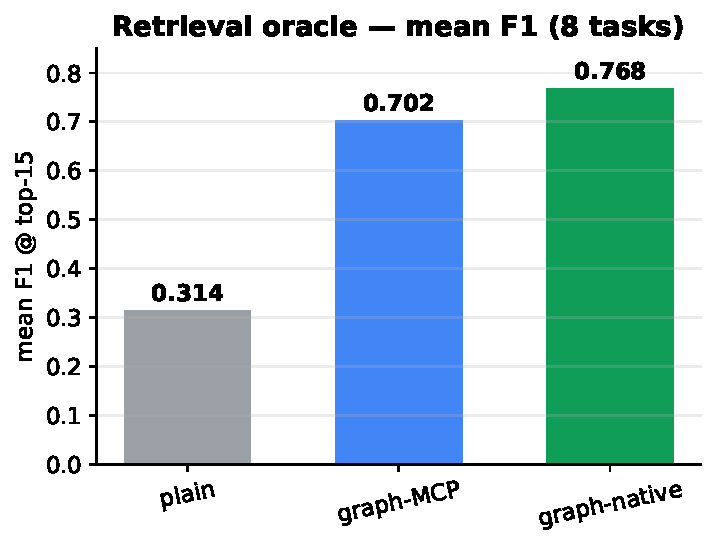
\includegraphics[width=\linewidth]{figs/retrieval_f1.pdf}
\end{minipage}\hfill
\begin{minipage}{0.44\linewidth}\small\raggedright
\textbf{Live validation.} On a 59-file ``firehose'' impact task (52 of them tests), the live
graph-native agent scored \native{F1 0.56 vs plain 0.52}, at \native{precision 1.00} and
\native{lower cost} (\$0.61 vs \$0.67) --- the oracle's prediction held end-to-end.\\[4pt]
plain collapses to \textbf{0.00} on data-flow / dead-code / refactor-triage: these are graph
traversals that text search cannot express.
\end{minipage}

\subsection{Cost}
\begin{center}
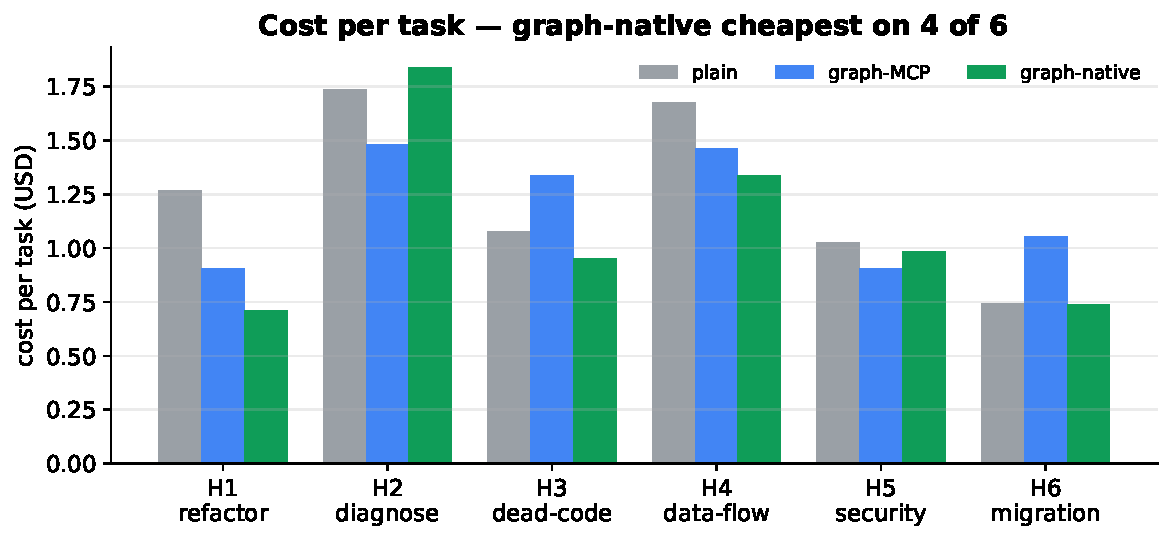
\includegraphics[width=0.9\linewidth]{figs/cost.pdf}
\end{center}
\figcap{Per-task cost. graph-native is cheapest on 4 of 6 tasks --- pre-computed retrieval shows up as fewer turns and lower spend.}

\subsection{Method integrity \& honest negatives}
\begin{itemize}
\item \textbf{Blind judging}, rubric-based, no tools/repo --- the judge grades text it cannot trace to a harness.
\item \textbf{A judge bug we caught \& fixed}: long code-bearing answers triggered judge refusals
  (a false 0.0); fixed via system-prompt role-pinning + fenced data + robust JSON extraction, re-verified.
\item \textbf{Negatives kept in, not hidden}: graph-MCP beats native on H2/H5; plain ties on H3/H5.
\item \textbf{Small $n$} (6 hardcore, 8 oracle tasks, 1 repo, 1 run/arm) --- directional, not a population estimate.
\item All evaluation was \textbf{additive}; no production code in the target repo was modified.
\end{itemize}

\vspace{6pt}{\color{rule}\hrule}\vspace{4pt}
{\footnotesize\color{plainc} Reproduce: \texttt{scripts/\{oracle-3harness,run-hardcore,agent-ab\}.mjs};
figures via \texttt{report/make\_figs.py}. Full write-ups in \texttt{results/}; captured traces in \texttt{runs/}.}

\end{document}
